\documentclass[12pt,letterpaper]{article}

\usepackage[spanish]{babel}
\usepackage[utf8]{inputenc}
\usepackage[T1]{fontenc}
\usepackage{csquotes}
\usepackage{caption}
\usepackage[style=apa, backend=biber, language=spanish]{biblatex}
\addbibresource{referencias.bib}
\usepackage{graphicx}
\usepackage[hidelinks]{hyperref}
\usepackage{pdflscape}

\usepackage{geometry}
\geometry{
  left=3cm,
  right=2cm,
  top=2cm,
  bottom=2cm
}

\usepackage{setspace}
\usepackage{parskip}
\usepackage{ragged2e}
\usepackage{float}
\usepackage{array}
\usepackage{tabularx}
\usepackage{booktabs}
\usepackage{longtable}
\usepackage{forest}
\usepackage{multicol}
\usepackage{verbatim}

\usepackage{tocloft}
\setlength{\parindent}{0pt}

\addto\captionsspanish{
  \renewcommand{\contentsname}{ÍNDICE GENERAL}
}

\setlength{\cftbeforetoctitleskip}{0pt}
\setlength{\cftbeforeloftitleskip}{0pt}
\setlength{\cftbeforelottitleskip}{0pt}
\setlength{\cftaftertoctitleskip}{12pt}
\setlength{\cftafterloftitleskip}{12pt}
\setlength{\cftafterlottitleskip}{12pt}

\renewcommand{\cfttoctitlefont}{\fontsize{12}{14}\selectfont\bfseries}
\renewcommand{\cftloftitlefont}{\fontsize{12}{14}\selectfont\bfseries}
\renewcommand{\cftlottitlefont}{\fontsize{12}{14}\selectfont\bfseries}

\usepackage{titlesec}

\titleformat{\section}[block]
  {\fontsize{12}{14}\selectfont\bfseries}
  {\thesection}
  {0.5em}
  {}
\titlespacing*{\section}{0pt}{6pt}{6pt}

\titleformat{\subsection}[block]
  {\fontsize{11}{13}\selectfont\bfseries}
  {\thesubsection}
  {0.5em}
  {}
\titlespacing*{\subsection}{0pt}{6pt}{6pt}

\titleformat{\subsubsection}[block]
  {\fontsize{11}{13}\selectfont\normalfont}
  {\thesubsubsection}
  {0.5em}
  {}
\titlespacing*{\subsubsection}{0pt}{6pt}{6pt}

\usepackage{fancyhdr}
\pagestyle{fancy}
\fancyhf{}
\fancyfoot[C]{\thepage}
\renewcommand{\headrulewidth}{0pt}
\setlength{\footskip}{24pt}

\AtBeginDocument{%
  \singlespacing
  \setlength{\parskip}{6pt}
  \justifying
}

\begin{document}

\begin{titlepage}
\centering
\vspace*{0cm}
\begin{minipage}[c]{0.18\textwidth}
  \centering
  \IfFileExists{logo_left.png}{
\includegraphics[width=0.8\textwidth]{logo_left.png}}{\rule{0pt}{2.8cm}}
\end{minipage}%
\hfill
\begin{minipage}[c]{0.64\textwidth}
  \centering
  {\fontsize{12}{15}\selectfont\bfseries
  UNIVERSIDAD MAYOR DE SAN SIMÓN\\[4pt]
  FACULTAD DE CIENCIAS Y TECNOLOGÍA\\[4pt]
  CARRERA DE INGENIERÍA INFORMÁTICA}
\end{minipage}%
\hfill
\begin{minipage}[c]{0.18\textwidth}
  \centering
  \IfFileExists{logo_right.png}{
\includegraphics[width=0.9\textwidth]{logo_right.png}}{\rule{0pt}{2.8cm}}
\end{minipage}

\vspace{2.5cm}

{\fontsize{16}{32}\selectfont\bfseries BUSCADOR SEMÁNTICO DEL SISTEMA DE ALOJAMIENTO TIPO AIRBNB}\\[0.4cm]
\vspace{0.5cm}

{\large{Modelo semántico para la gestión de alojamientos, reservas y reputación de usuarios}}\\[0.3cm]

\vspace{0.5cm}

\setstretch{1.6}
{\large
\textbf{Materia:} Web Semánticas\\[8pt]
\textbf{Docente:} Ing. Erika Patricia Rodríguez Bilbao\\[8pt]
\textbf{Integrantes:}\\[6pt]
Gil Rivera Brisa Valeria\\
Sirpa Escalera Steve Jason\\
Castro Tejada Steven Lisandro\\
Rafael Montaño Aaron David\\
Velasquez Vela Marcos\\[8pt]
\textbf{Grupo:} 27\\[8pt]
}

\vfill

{\large\bfseries COCHABAMBA -- BOLIVIA}\\[4pt]
{\normalsize Junio -- 2026}

\end{titlepage}

\clearpage
\thispagestyle{empty}
\tableofcontents
\clearpage


\clearpage
\setcounter{page}{1}

\section{INTRODUCCIÓN}

La Web Semántica propone un cambio de enfoque en la publicación y recuperación de
información en la Web: los datos dejan de ser únicamente documentos legibles por
personas y pasan a representarse también como conocimiento formal interpretable por
máquinas \parencite{berners-lee2001}. Este enfoque se sustenta en estándares del W3C
como RDF para la representación de grafos de conocimiento, RDFS y OWL para la
definición de vocabularios y ontologías, y SPARQL para la consulta declarativa sobre
esos grafos.

En plataformas de alojamiento temporal tipo Airbnb, la necesidad de representar
conocimiento semántico es especialmente evidente. La decisión de reserva no depende de
un solo atributo, sino de combinaciones entre tipo de propiedad, rango de precio,
ubicación, amenidades, perfil del viajero y propósito del viaje. Una consulta como
``quiero un departamento tranquilo, con Wi-Fi, adecuado para trabajo remoto y cercano a
una universidad'' contiene relaciones implícitas entre conceptos que un buscador basado
solo en filtros discretos no modela ni explota adecuadamente.

En este contexto, el presente trabajo desarrolla un buscador semántico para el dominio
de alojamiento temporal. La solución se apoya en una ontología OWL/RDF propia cargada
en Apache Jena Fuseki, sobre la cual se ejecutan consultas SPARQL para recuperar y
ordenar resultados. El sistema no se limita a buscar coincidencias textuales, sino que
combina restricciones duras sobre precio, capacidad o ciudad con criterios semánticos
relacionados con amenidades, perfiles de huésped y propósito del viaje.

Un requisito central del enunciado fue la integración con DBpedia. En la solución
implementada, esta integración se materializa mediante el enriquecimiento de la
ontología local con enlaces \texttt{owl:sameAs} y \texttt{owl:equivalentClass} hacia
recursos de DBpedia vinculados con tipos de alojamiento, amenidades y ciudades de
Bolivia. Este enfoque permite incorporar conocimiento geográfico real y, al mismo
tiempo, mantener una demostración estable en entorno local sobre Fuseki sin depender de
la disponibilidad del \textit{endpoint} público en cada consulta.

Otro requisito explícito fue la multilingüidad. Por ello, la ontología fue enriquecida
con anotaciones \texttt{rdfs:label} y \texttt{rdfs:comment} en tres idiomas:
español, inglés y francés. Esta representación permite reutilizar un único grafo RDF
para distintas interfaces de usuario y demuestra un uso correcto de las capacidades de
internacionalización propias de RDF/OWL.

La aplicación resultante fue implementada con Next.js como capa de presentación y de
servicios, Fuseki como \textit{triple store}, Bun como entorno de ejecución y un módulo
de procesamiento lingüístico para interpretar consultas en lenguaje natural. El sistema final ofrece una
interfaz web con navegación multilingüe, resultados visuales por tarjetas y búsqueda
semántica sobre una ontología consistente y validada.

El informe se organiza en cinco bloques principales: introducción y objetivos del
trabajo, marco teórico de las tecnologías de Web Semántica utilizadas, marco
referencial del dominio seleccionado, sección de ingeniería con la descripción de la
ontología, la arquitectura y las pruebas del prototipo, y finalmente las conclusiones
obtenidas a partir del desarrollo realizado.


\clearpage
\section{OBJETIVOS}

\subsection{Objetivo General}

Desarrollar un metabuscador semántico de alojamientos temporales inspirado en
plataformas de intermediación tipo Airbnb, basado en una ontología OWL del
dominio, integrado con la base de conocimiento enlazada DBpedia e incorporando
soporte multilingüe mediante anotaciones \texttt{rdfs:label}, con el fin de
demostrar la capacidad de las tecnologías de la Web Semántica para la
representación y recuperación expresiva de información en dominios complejos.

\subsection{Objetivos Específicos}

\begin{itemize}

      \item Modelar formalmente el dominio de los alojamientos temporales mediante una
      ontología OWL que represente propiedades de hospedaje, amenidades, zonas
      geográficas, perfiles de huésped, propósitos de viaje y políticas de reserva,
      estableciendo relaciones semánticas y restricciones lógicas entre los
      conceptos del sistema.

      \item Diseñar un conjunto de preguntas de competencia que representen los
      principales escenarios de búsqueda dentro del dominio y que permitan evaluar
      la capacidad de la ontología para responder consultas complejas mediante el
      lenguaje SPARQL.

      \item Implementar consultas SPARQL capaces de resolver las preguntas de
      competencia definidas, combinando múltiples criterios de búsqueda relacionados
      con ubicación geográfica, características del alojamiento, disponibilidad de
      amenidades y contexto del viaje.

      \item Integrar la ontología con la base de conocimiento enlazada DBpedia con el
      fin de incorporar información geográfica real sobre ciudades, zonas urbanas y
      puntos de interés del territorio boliviano, enriqueciendo así la base de
      conocimiento del sistema.

      \item Incorporar soporte multilingüe dentro de la ontología mediante
      anotaciones \texttt{rdfs:label} con etiquetas de idioma, permitiendo que los
      conceptos, propiedades e instancias del modelo puedan representarse y
      recuperarse en diferentes lenguajes.

      \item Verificar la consistencia lógica del modelo ontológico utilizando un
      razonador OWL integrado en Protégé, garantizando la coherencia de la jerarquía
      de clases, las relaciones semánticas y las restricciones definidas en el
      modelo.

      \item Implementar un prototipo de aplicación web que permita a los usuarios
      explorar y buscar alojamientos temporales mediante una interfaz similar a las
      plataformas de reservas en línea o marketplaces de hospedaje. La interfaz
      permitirá visualizar propiedades, aplicar filtros de búsqueda y consultar
      resultados de forma intuitiva, mientras que el procesamiento de las consultas
      se realizará internamente sobre la base de conocimiento semántica mediante
      consultas SPARQL.

\end{itemize}

\clearpage
\section{MARCO TEÓRICO}

\subsection{Web Semántica}

La Web Semántica es una extensión de la Web tradicional orientada a que los datos no
solo sean publicados para consumo humano, sino también descritos de manera formal para
ser interpretados por agentes de software \parencite{berners-lee2001}. Su objetivo no
es reemplazar la Web documental, sino complementarla con una capa semántica que permita
representar entidades, relaciones, restricciones y reglas de inferencia sobre los
recursos disponibles.

Desde el punto de vista arquitectónico, la Web Semántica se apoya en una pila de
estándares del W3C. En la base se encuentran los URI como identificadores globales de
recursos; sobre ellos, RDF como modelo de representación; posteriormente, RDFS y OWL
como lenguajes de descripción y formalización de vocabularios; y finalmente SPARQL
como lenguaje de consulta sobre grafos RDF. Gracias a esta pila tecnológica es posible
publicar conocimiento de manera interoperable y vincularlo con otras fuentes dentro del
ecosistema de \textit{Linked Data}.

\subsection{RDF como modelo de representación}

El \textit{Resource Description Framework} (RDF) es el modelo de datos básico de la Web
Semántica \parencite{w3c-rdf2014}. RDF expresa la información mediante triples de la
forma sujeto--predicado--objeto. El sujeto representa el recurso descrito, el
predicado expresa una propiedad o relación, y el objeto representa el valor de esa
propiedad, ya sea otro recurso o un literal.

Un conjunto de triples conforma un grafo RDF. Esta estructura es flexible, extensible y
adecuada para dominios complejos, ya que permite agregar nuevos hechos sin rediseñar el
modelo completo. En aplicaciones como la desarrollada en este trabajo, RDF es
particularmente útil porque permite integrar en un mismo grafo información sobre
propiedades, amenidades, perfiles de huésped, zonas geográficas y recursos enlazados a
fuentes externas como DBpedia.

\subsection{RDFS y anotaciones semánticas}

RDF Schema extiende RDF con construcciones básicas para describir tipos y jerarquías
\parencite{w3c-rdfs2014}. Entre sus elementos más importantes se encuentran
\texttt{rdfs:Class}, \texttt{rdfs:subClassOf}, \texttt{rdfs:domain} y
\texttt{rdfs:range}. Estas construcciones permiten definir clases, organizar
subsunciones entre ellas y restringir el uso de las propiedades.

Además, RDFS introduce anotaciones como \texttt{rdfs:label} y \texttt{rdfs:comment},
que permiten asociar nombres legibles y descripciones textuales a recursos. Estas
anotaciones son especialmente relevantes para el presente proyecto, ya que constituyen
la base del soporte multilingüe implementado en la ontología mediante etiquetas en
español, inglés y francés.

\subsection{Ontologías OWL}

Una ontología es una especificación formal de un dominio de conocimiento, donde se
declaran conceptos, relaciones, individuos y restricciones lógicas. OWL es el estándar
del W3C para la definición de ontologías sobre RDF \parencite{w3c-owl2012}. Frente a la
expresividad limitada de RDFS, OWL incorpora constructores más ricos para representar
disjunciones, equivalencias, restricciones existenciales, cardinalidades y axiomas
lógicos con semántica formal basada en lógica descriptiva.

En OWL, una ontología puede incluir:

\begin{itemize}
  \item \textbf{Clases}, que agrupan individuos con características comunes.
  \item \textbf{Propiedades de objeto}, que vinculan individuos con otros individuos.
  \item \textbf{Propiedades de dato}, que vinculan individuos con literales.
  \item \textbf{Individuos}, que representan instancias concretas del dominio.
  \item \textbf{Axiomas}, que describen restricciones, equivalencias, disjunciones o
  condiciones de pertenencia.
\end{itemize}

La ontología desarrollada en esta práctica fue modelada en OWL 2 DL, ya que este
perfil ofrece un equilibrio adecuado entre expresividad y decidibilidad. Gracias a ello,
el modelo puede ser verificado por un razonador automático y al mismo tiempo mantener
capacidad suficiente para representar el dominio de alojamientos temporales.

\subsection{SPARQL como lenguaje de consulta}

SPARQL es el lenguaje estándar para consultar grafos RDF \parencite{w3c-sparql2013}.
Una consulta SPARQL declara patrones de triples que deben satisfacerse en el grafo de
conocimiento y puede complementarse con filtros, uniones, agregaciones, ordenamiento y
agrupamiento de resultados.

En el contexto del presente trabajo, SPARQL se utiliza en dos niveles. Primero, como
mecanismo principal de recuperación sobre el dataset local cargado en Fuseki. Segundo,
como medio para demostrar interoperabilidad con DBpedia mediante consultas federadas con
la cláusula \texttt{SERVICE}. Aunque la aplicación final se apoya sobre un dataset local
enriquecido para mejorar estabilidad y rendimiento, el uso de \texttt{SERVICE} sigue
siendo relevante como evidencia de integración con una base de conocimiento enlazada.

\subsection{Lógica de Descripción y razonamiento}

La base formal de OWL 2 DL se encuentra en la Lógica de Descripción. Este marco permite
definir conceptos de manera precisa y habilita inferencias automáticas sobre la
ontología \parencite{baader2003}. A partir de un conjunto de axiomas, un razonador
puede verificar consistencia, clasificar jerarquías de clases y determinar la
pertenencia de individuos a conceptos derivados.

El razonamiento automático es importante en ontologías aplicadas porque permite detectar
errores conceptuales tempranos. Por ejemplo, si dos clases son declaradas disjuntas, un
individuo no debería pertenecer simultáneamente a ambas; si esto ocurre, el razonador lo
identifica como inconsistencia. En este proyecto se utilizó HermiT para verificar que la
ontología modelada no incurre en contradicciones lógicas \parencite{glimm2014}.

\subsection{Ingeniería de ontologías y preguntas de competencia}

La ingeniería de ontologías es el proceso metodológico mediante el cual se construyen y
mantienen modelos formales de conocimiento. Una práctica central en este proceso es la
definición de \textit{preguntas de competencia}: consultas representativas del dominio
que la ontología debe ser capaz de responder. Estas preguntas permiten validar la
cobertura conceptual del modelo y orientar su diseño desde necesidades reales de uso.

En el dominio de alojamiento temporal, las preguntas de competencia suelen combinar
ciudad, rango de precio, tipo de propiedad, amenidades, perfil del viajero y propósito
de la estadía. Por ello, la ontología no debe limitarse a almacenar atributos, sino que
debe representar relaciones semánticas que permitan responder consultas compuestas de
forma coherente.

\subsection{Protégé y HermiT como entorno de modelado}

Protégé es el entorno de edición ontológica más utilizado en proyectos de Web
Semántica \parencite{musen2015}. Permite modelar clases, propiedades, restricciones e
individuos, y además ofrece integración con razonadores como HermiT. En este trabajo,
Protégé fue utilizado para el diseño inicial de la ontología y HermiT para la
verificación de consistencia y revisión de la jerarquía lógica.

\subsection{DBpedia como base de conocimiento enlazada}

DBpedia es una de las bases de conocimiento enlazadas más representativas del ecosistema
de \textit{Linked Data}. Extrae información estructurada de Wikipedia y la publica en
RDF, con millones de entidades y etiquetas multilingües \parencite{lehmann2015}. Su
utilidad en este proyecto radica en que provee referencias geográficas reales para el
territorio boliviano y recursos equivalentes para conceptos del dominio como tipos de
alojamiento o amenidades.

La integración con DBpedia puede realizarse de varias maneras: mediante consultas
federadas en tiempo de ejecución, mediante descarga previa de subconjuntos RDF o a
través de enlaces semánticos entre recursos locales y remotos. En la solución final se
priorizó este último enfoque, incorporando \texttt{owl:sameAs} y
\texttt{owl:equivalentClass} en la ontología local, lo que hace más estable la
demostración sobre Fuseki y, al mismo tiempo, conserva la trazabilidad hacia los
recursos de DBpedia utilizados.

\subsection{Representación multilingüe en ontologías}

Una de las ventajas más importantes de RDF/OWL es que la multilingüidad puede
representarse directamente mediante literales etiquetados por idioma. La forma más
simple y estándar consiste en utilizar \texttt{rdfs:label} y \texttt{rdfs:comment}
con etiquetas como \texttt{@es}, \texttt{@en} o \texttt{@fr} \parencite{w3c-rdf2014}.

Este enfoque tiene varias ventajas técnicas: evita duplicar la ontología, mantiene una
única identidad semántica para cada recurso y permite seleccionar el idioma requerido en
las consultas SPARQL mediante la función \texttt{LANG()} o estrategias de fallback.
Precisamente esta capacidad fue aprovechada en el proyecto para servir resultados en
español, inglés y francés desde un único dataset OWL cargado en Fuseki.


\clearpage
\section{MARCO REFERENCIAL}

\subsection{Dominio de conocimiento seleccionado}

El dominio elegido para la práctica es el de los sistemas de alojamiento temporal de
intermediación tipo Airbnb. Este dominio involucra propiedades heterogéneas,
restricciones de uso, amenidades, perfiles de viajeros, finalidades de estadía y un
contexto geográfico que condiciona fuertemente la decisión de reserva. En consecuencia,
se trata de un escenario adecuado para aplicar modelado ontológico y recuperación de
información basada en semántica.

Una propiedad no puede analizarse únicamente por su precio o por su tipo. La decisión de
un usuario depende también de factores como la capacidad máxima, la cercanía a zonas
urbanas o puntos de interés, la disponibilidad de Wi-Fi, cocina o piscina, y la
compatibilidad con perfiles de viaje como pareja, familia, estudiante o ejecutivo. Esta
interdependencia entre atributos hace que el dominio sea más cercano a un problema de
representación de conocimiento que a un simple catálogo tabular.

\subsection{Justificación del dominio}

El dominio seleccionado es pertinente por cuatro razones principales:

\begin{itemize}
  \item \textbf{Complejidad conceptual}. El dominio incluye entidades distintas pero
  interrelacionadas: propiedades, amenidades, perfiles de huésped, propósitos de viaje,
  políticas y zonas geográficas.

  \item \textbf{Necesidad de consultas compuestas}. Las búsquedas reales combinan más de
  un criterio y requieren relacionar conceptos que no siempre se expresan como filtros
  exactos.

  \item \textbf{Disponibilidad de datos enlazados}. DBpedia provee recursos geográficos
  y etiquetas multilingües aprovechables para enriquecer el modelo local.

  \item \textbf{Valor demostrativo del multilingüismo}. El dominio es adecuado para
  mostrar internacionalización semántica, ya que las mismas entidades pueden presentarse
  correctamente en varios idiomas sin duplicar la ontología.
\end{itemize}

\subsection{Problema de los buscadores convencionales}

Los buscadores convencionales en plataformas de alojamiento suelen apoyarse en filtros
discretos y coincidencias literales. Este enfoque funciona para atributos explícitos,
pero falla cuando el usuario expresa necesidades semánticas. Por ejemplo, ``alojamiento
adecuado para trabajo remoto'' puede implicar Wi-Fi, espacio de trabajo, zona tranquila
o perfil ejecutivo; ``propiedad conveniente para estudiantes'' puede implicar precio
moderado, cercanía a universidades y estadías funcionales.

Cuando el modelo de datos no representa esas relaciones de forma explícita, el sistema
solo puede responder por coincidencias exactas o por reglas externas difíciles de
mantener. Una ontología permite, en cambio, representar el dominio como una red de
conceptos vinculados y consultables declarativamente mediante SPARQL.

\subsection{Conceptualización del dominio}

El análisis del dominio permitió identificar los conceptos centrales que estructuran el
modelo ontológico:

\begin{itemize}
  \item \textbf{Propiedad}. Representa la unidad ofertada, con atributos como nombre,
  descripción, precio por noche, capacidad máxima, calificación e imagen.

  \item \textbf{Tipo de propiedad}. Especializa el inventario en apartamento, casa,
  habitación privada, habitación compartida y villa.

  \item \textbf{Amenidad}. Modela servicios o equipamientos relevantes para la decisión
  de reserva, por ejemplo Wi-Fi, piscina, desayuno o espacio de trabajo.

  \item \textbf{Zona geográfica}. Describe la localización del alojamiento en una ciudad
  y una zona concreta, incorporando el contexto urbano del dominio.

  \item \textbf{Punto de interés}. Representa lugares próximos relevantes para la
  búsqueda, como plazas, universidades, terminales, hospitales o centros comerciales.

  \item \textbf{Perfil de huésped}. Describe el tipo de usuario o de grupo al que puede
  resultar más afín una propiedad.

  \item \textbf{Propósito de viaje}. Permite distinguir entre turismo, trabajo,
  estudios, congresos o reubicación.

  \item \textbf{Política}. Modela reglas de reserva o uso, necesarias para reflejar
  restricciones del dominio.
\end{itemize}

\subsection{Preguntas de competencia}

Las preguntas de competencia fueron definidas para asegurar que la ontología responda a
consultas representativas del problema. Entre las más relevantes se encuentran:

\begin{itemize}
  \item ¿Qué propiedades existen en una ciudad determinada y dentro de un rango de
  precio?
  \item ¿Qué alojamientos poseen amenidades específicas como Wi-Fi, piscina, cocina o
  espacio de trabajo?
  \item ¿Qué propiedades son compatibles con perfiles como familia, pareja, estudiantes
  o ejecutivos?
  \item ¿Qué alojamientos satisfacen simultáneamente restricciones de ubicación,
  capacidad, amenidades y contexto del viaje?
  \item ¿Cómo presentar la misma propiedad en distintos idiomas a partir de un único
  grafo RDF?
\end{itemize}

Estas preguntas guiaron tanto la estructura de la ontología como la implementación de
las consultas SPARQL y del prototipo web.

\subsection{Terminología base del dominio}

La terminología utilizada en el modelo fue refinada a partir del análisis del dominio,
de vocabularios de alojamiento y de las necesidades de recuperación expresadas por las
preguntas de competencia.

\begin{longtable}{|p{3.3cm}|p{5.2cm}|p{5.2cm}|}
\hline
\textbf{Área} & \textbf{Término en español} & \textbf{Equivalente operativo en inglés} \\
\hline
\endfirsthead
\hline
\textbf{Área} & \textbf{Término en español} & \textbf{Equivalente operativo en inglés} \\
\hline
\endhead
\hline
\multicolumn{3}{|r|}{\textit{Continúa en la siguiente página}} \\
\hline
\endfoot
\hline
\endlastfoot
Tipos de propiedad & Apartamento & Apartment \\
\hline
Tipos de propiedad & Casa & House \\
\hline
Tipos de propiedad & Habitación privada & Private room \\
\hline
Tipos de propiedad & Habitación compartida & Shared room \\
\hline
Tipos de propiedad & Villa & Villa \\
\hline
Amenidades & Wi-Fi & Wi-Fi \\
\hline
Amenidades & Cocina & Kitchen \\
\hline
Amenidades & Piscina & Swimming pool \\
\hline
Amenidades & Lavandería & Laundry \\
\hline
Amenidades & Desayuno & Breakfast \\
\hline
Amenidades & Espacio de trabajo & Workspace \\
\hline
Ubicación & Ciudad & City \\
\hline
Ubicación & Zona geográfica & Geographic area \\
\hline
Ubicación & Punto de interés & Point of interest \\
\hline
Perfil & Pareja & Couple \\
\hline
Perfil & Familia & Family \\
\hline
Perfil & Grupo estudiantil & Student group \\
\hline
Perfil & Ejecutivo & Executive traveler \\
\hline
Contexto & Viaje de trabajo & Business trip \\
\hline
Contexto & Viaje de estudios & Study trip \\
\hline
Contexto & Viaje vacacional & Vacation trip \\
\hline
Política & Política flexible & Flexible policy \\
\hline
Política & Política corporativa & Corporate policy \\
\hline
Política & Política para eventos & Events policy \\
\hline
Búsqueda & Consulta semántica & Semantic query \\
\hline
Búsqueda & Ranking de relevancia & Relevance ranking \\
\hline
Búsqueda & Filtros estructurados & Structured filters \\
\hline
\end{longtable}

\subsection{Relación con vocabularios y recursos existentes}

La ontología propia no fue construida aislada del ecosistema de Web Semántica. Se tomó
como referencia la existencia de vocabularios generales y específicos del dominio, así
como recursos disponibles en DBpedia. No obstante, dado que el objetivo de la práctica
era construir un modelo propio orientado a un buscador semántico concreto, se optó por
una ontología de dominio ajustada al caso de uso, y no por una simple reutilización
directa de un vocabulario externo completo.

Esta decisión permitió adaptar el modelo a necesidades reales del prototipo, como el
ranking semántico, los perfiles de huésped y la localización de zonas bolivianas, al
mismo tiempo que se preservó interoperabilidad mediante enlaces a recursos de DBpedia y
anotaciones multilingües estándar.

\subsection{Integración conceptual con DBpedia}

La integración con DBpedia se centró en los recursos más útiles y defendibles para el
dominio: tipos de alojamiento, amenidades y ciudades bolivianas. El criterio aplicado
fue seleccionar entidades de uso directo dentro del proyecto, evitando incorporar un
volumen excesivo de referencias irrelevantes para la demostración.

En términos prácticos, la integración se realizó mediante dos mecanismos:

\begin{itemize}
  \item \textbf{Alineación semántica}. Se añadieron enlaces
  \texttt{owl:equivalentClass} para clases como \texttt{Apartamento}, \texttt{Casa},
  \texttt{Villa} y \texttt{HabitacionPrivada}/\texttt{HabitacionCompartida} con sus
  equivalentes en DBpedia.

  \item \textbf{Enlace de individuos}. Se añadieron enlaces \texttt{owl:sameAs} para
  amenidades y ciudades bolivianas relevantes, aprovechando los recursos de DBpedia como
  referencia externa normalizada.
\end{itemize}

Este enfoque satisface el requisito de conexión con DBpedia y, al mismo tiempo, mejora
la robustez de la solución al mantener la operación principal sobre un dataset local en
Fuseki.

\subsection{Multilingüidad del dominio}

El enunciado exigía incorporar multilingüidad. En lugar de duplicar propiedades como
\texttt{nombreEn} o \texttt{descripcionEn}, se adoptó la estrategia recomendada en RDF:
etiquetar cada recurso con \texttt{rdfs:label} y \texttt{rdfs:comment} en varios
idiomas. Esto permite que el mismo individuo conserve identidad semántica única y sea
presentado en español, inglés o francés según la interfaz de usuario o la consulta
SPARQL ejecutada.

La elección del francés como tercer idioma, además de español e inglés, fortalece la
demostración de que la solución no fue diseñada solo para un caso bilingüe puntual, sino
para un esquema escalable de internacionalización semántica.


\clearpage
\section{INGENIERÍA DEL SISTEMA}

\subsection{Descripción general de la solución}

La solución implementada corresponde a un buscador semántico de alojamientos temporales
construido sobre una ontología OWL/RDF cargada en Apache Jena Fuseki. La interfaz web
permite realizar búsquedas en lenguaje natural, interpretar criterios estructurados y
presentar resultados en tres idiomas. La arquitectura fue pensada para que la ontología
sea el núcleo del sistema y no un artefacto secundario: tanto la recuperación de
resultados como la internacionalización dependen directamente del grafo semántico.

Desde el punto de vista de ejecución, el sistema combina tres componentes principales:
una base de conocimiento ontológica, un \textit{triple store} con endpoint SPARQL y una
aplicación web que consume ese endpoint. El enriquecimiento con DBpedia se integra en la
propia ontología mediante alineaciones y enlaces semánticos, lo que permite mantener la
operación principal en local sobre Fuseki y, a la vez, demostrar interoperabilidad con
Linked Data.

\subsection{Arquitectura implementada}

La arquitectura real del proyecto se organiza en tres capas:

\begin{itemize}
  \item \textbf{Capa de conocimiento}. Contiene la ontología
  \texttt{ontology/Airbnb.owl}, donde se definen clases, propiedades, axiomas,
  individuos, etiquetas multilingües y enlaces a DBpedia.

  \item \textbf{Capa de persistencia y consulta}. Está implementada con Apache Jena
  Fuseki, que expone el endpoint SPARQL del dataset local \texttt{airbnb}. Esta capa es
  responsable de almacenar el grafo RDF y responder las consultas ejecutadas por la
  aplicación.

  \item \textbf{Capa de aplicación}. Se implementó con Next.js 16 y React 19. Esta
  capa interpreta la consulta del usuario, llama a Fuseki, aplica ranking semántico y
  renderiza los resultados en la interfaz web.
\end{itemize}

\begin{table}[H]
\centering
\caption{Tecnologías utilizadas en la implementación}
\begin{tabular}{|p{3.8cm}|p{4.0cm}|p{6.2cm}|}
\hline
\textbf{Componente} & \textbf{Tecnología} & \textbf{Uso dentro del proyecto} \\
\hline
Modelado ontológico & Protégé 5.6 + HermiT & Diseño de la ontología, edición de clases, propiedades e individuos, y validación de consistencia lógica. \\
\hline
Representación semántica & OWL 2 DL + RDF/XML & Formalización del dominio y serialización principal del conocimiento. \\
\hline
Consulta semántica & SPARQL 1.1 & Recuperación de propiedades, amenidades, perfiles y filtrado por idioma. \\
\hline
Triple store & Apache Jena Fuseki & Carga del dataset local y exposición del endpoint SPARQL. \\
\hline
Aplicación web & Next.js 16 + React 19 & Interfaz del buscador, rutas por idioma y consumo del backend semántico. \\
\hline
Runtime & Bun & Ejecución del proyecto web y gestión de dependencias. \\
\hline
Procesamiento lingüístico & Módulo de procesamiento de consultas & Interpretación de consultas en lenguaje natural y transformación hacia filtros estructurados. \\
\hline
Base enlazada externa & DBpedia & Referencia para tipos de alojamiento, amenidades y ciudades bolivianas. \\
\hline
Imágenes & Unsplash & Fotografías referenciales incluidas en la ontología mediante URL. \\
\hline
\end{tabular}
\end{table}

\subsection{Estructura ontológica resultante}

La ontología desarrollada no modela un concepto genérico de ``alojamiento'' abstracto
desconectado del proyecto, sino un dominio operativo orientado a la recuperación
semántica de propiedades. El eje principal del modelo es la clase \texttt{Propiedad},
de la cual derivan los tipos concretos que el usuario visualiza y consulta.

Las clases más importantes del modelo son:

\begin{itemize}
  \item \texttt{Propiedad}
  \item \texttt{AlojamientoCompleto}
  \item \texttt{AlojamientoHabitacion}
  \item \texttt{Apartamento}
  \item \texttt{Casa}
  \item \texttt{HabitacionPrivada}
  \item \texttt{HabitacionCompartida}
  \item \texttt{Villa}
  \item \texttt{Amenidad}
  \item \texttt{ZonaGeografica}
  \item \texttt{PuntoInteres}
  \item \texttt{PerfilHuesped}
  \item \texttt{PropositoViaje}
  \item \texttt{Politica}
\end{itemize}

Las relaciones fundamentales del modelo se expresan mediante propiedades de objeto como
\texttt{tieneAmenidad}, \texttt{compatibleCon}, \texttt{ubicadaEn},
\texttt{tienePropositoViaje}, \texttt{tienePuntoInteres} y \texttt{tienePolitica}. A
ello se suman propiedades de dato para nombre, descripción, precio, capacidad,
calificación, ciudad, zona e imagen referencial.

\begin{table}[H]
\centering
\caption{Resumen estructural de la ontología implementada}
\begin{tabular}{|p{7cm}|c|}
\hline
\textbf{Elemento} & \textbf{Cantidad} \\
\hline
Clases OWL & 14 \\
\hline
Propiedades de objeto & 6 \\
\hline
Propiedades de dato & 53 \\
\hline
Individuos nombrados & 140 \\
\hline
Propiedades publicadas en el catálogo & 62 \\
\hline
Etiquetas \texttt{rdfs:label} en español & 216 \\
\hline
Etiquetas \texttt{rdfs:label} en inglés & 216 \\
\hline
Etiquetas \texttt{rdfs:label} en francés & 216 \\
\hline
Enlaces \texttt{owl:sameAs} a DBpedia & 14 \\
\hline
Enlaces \texttt{owl:equivalentClass} & 5 \\
\hline
\end{tabular}
\end{table}

\subsection{Población del dominio e instancias}

La ontología fue poblada con un catálogo sintético pero coherente con el dominio de
alojamiento temporal. Se definieron 62 propiedades publicables distribuidas entre
apartamentos, casas, habitaciones privadas, habitaciones compartidas y villas. Además,
se añadieron 14 amenidades, 10 perfiles de huésped, 10 políticas, 10 propósitos de
viaje, 17 puntos de interés y 17 zonas geográficas.

La población de la ontología no se limita a datos nominales. Cada propiedad incorpora
atributos operativos relevantes para la búsqueda, como precio por noche, capacidad,
calificación, descripción e imagen. Esto permitió que el prototipo web no fuera solo una
demostración de consultas semánticas, sino una aplicación navegable con resultados
visuales completos.

\subsection{Restricciones y consistencia lógica}

La ontología fue diseñada cuidando la coherencia interna entre jerarquías y relaciones.
Se declararon clases disjuntas cuando correspondía, por ejemplo entre
\texttt{HabitacionPrivada} y \texttt{HabitacionCompartida}, y se definieron dominios y
rangos para las propiedades principales. Esto reduce ambigüedades y evita que una misma
relación sea utilizada sobre conceptos incompatibles.

La validación se realizó con HermiT desde Protégé. El razonador confirmó la ausencia de
contradicciones lógicas y permitió verificar que la estructura de clases es coherente
con los axiomas definidos. Esta verificación es importante porque garantiza que el
conocimiento cargado en Fuseki no contiene errores semánticos que afecten la consulta o
la interpretación del dominio.

\subsection{Integración real con DBpedia}

El requisito del enunciado relativo a DBpedia se resolvió enriqueciendo el grafo local
con enlaces semánticos hacia recursos de DBpedia utilizados directamente por el sistema.
Esta solución evita depender del endpoint público en cada búsqueda, pero preserva la
referencia formal a una base de conocimiento enlazada externa.

\subsubsection{Alineación de clases}

Las clases de tipos de propiedad se enlazaron con recursos de DBpedia mediante
\texttt{owl:equivalentClass}. Se utilizaron como referencia los recursos
\texttt{Apartment} \parencite{dbpedia_apartment}, \texttt{House}
\parencite{dbpedia_house}, \texttt{Villa} \parencite{dbpedia_villa} y
\texttt{Room} \parencite{dbpedia_room}.

\begin{verbatim}
<owl:Class rdf:about=".../Apartamento">
    <owl:equivalentClass rdf:resource="http://dbpedia.org/ontology/Apartment"/>
</owl:Class>
\end{verbatim}

\subsubsection{Alineación de amenidades}

Las amenidades más relevantes del dominio fueron enlazadas mediante
\texttt{owl:sameAs} con recursos de DBpedia, entre ellos Wi-Fi
\parencite{dbpedia_wifi}, Kitchen \parencite{dbpedia_kitchen}, Air conditioning
\parencite{dbpedia_air_conditioning}, Parking \parencite{dbpedia_parking}, Swimming
pool \parencite{dbpedia_swimming_pool}, Laundry \parencite{dbpedia_laundry}, Breakfast
\parencite{dbpedia_breakfast} y Cleaning \parencite{dbpedia_cleaning}. Esta decisión
fortalece la semántica del grafo y documenta explícitamente qué conceptos del dominio se
alinean con conocimiento enlazado externo.

\subsubsection{Alineación geográfica}

Las principales ciudades bolivianas utilizadas por el catálogo se enlazaron con DBpedia
mediante \texttt{owl:sameAs}: Cochabamba \parencite{dbpedia_cochabamba}, La Paz
\parencite{dbpedia_lapaz}, Santa Cruz de la Sierra
\parencite{dbpedia_santacruz}, Sucre \parencite{dbpedia_sucre} y Tarija
\parencite{dbpedia_tarija}. Estas alineaciones permiten justificar el origen externo del
componente geográfico y aprovechar recursos con etiquetas multilingües ya consolidadas.

\subsubsection{Consulta de interoperabilidad}

Aunque el flujo principal de la aplicación trabaja sobre un dataset local en Fuseki, se
definió también una consulta federada de validación con \texttt{SERVICE} para demostrar
la conexión con el endpoint público de DBpedia. Esta consulta no es el mecanismo central
del buscador en producción local, pero sí constituye evidencia de interoperabilidad con
Linked Data.

\begin{verbatim}
SELECT ?zona ?etiquetaDBpedia
WHERE {
  ?zona owl:sameAs ?recursoDBpedia .
  SERVICE <https://dbpedia.org/sparql> {
    ?recursoDBpedia rdfs:label ?etiquetaDBpedia .
    FILTER(LANG(?etiquetaDBpedia) = "es")
  }
}
\end{verbatim}

\subsection{Implementación del soporte multilingüe}

La multilingüidad no se resolvió duplicando entidades ni manteniendo tres catálogos
separados. La estrategia adoptada fue enriquecer la ontología con \texttt{rdfs:label} y
\texttt{rdfs:comment} en español, inglés y francés para clases, amenidades, zonas,
perfiles y propiedades publicadas. De esta manera, un mismo recurso RDF conserva una
identidad única y solo cambia su representación textual según el idioma solicitado.

En la capa SPARQL se implementó selección por idioma con fallback. La aplicación intenta
obtener primero el label o comment del idioma activo; si no existe, busca en otro idioma
disponible y finalmente cae a los campos textuales heredados del modelo original. Este
patrón mejora robustez y evita dejar resultados vacíos en caso de que alguna traducción
no exista todavía.

La interfaz web consume el mismo dataset para rutas \texttt{/es}, \texttt{/en} y
\texttt{/fr}. Esta decisión demuestra que la multilingüidad está implementada en la
capa semántica y no solo en textos estáticos de la interfaz.

\subsection{Motor de búsqueda y procesamiento de consultas}

El flujo de búsqueda se implementa en dos etapas. Primero, la consulta en lenguaje
natural es interpretada por un módulo de procesamiento lingüístico, que la transforma en filtros
estructurados sobre ciudad, zona, tipo de propiedad, amenidades, capacidad o rango de
precio. Segundo, esos filtros se aplican sobre Fuseki mediante consultas SPARQL y un
proceso de ranking adicional en la capa de aplicación.

Los filtros duros, como ciudad, precio o capacidad, se resuelven directamente en SPARQL.
Posteriormente, los resultados son reordenados considerando coincidencias semánticas con
amenidades, perfiles y palabras clave. Esta estrategia híbrida combina precisión en la
restricción del conjunto de candidatos con flexibilidad en la presentación de resultados
más relevantes.

El flujo operacional de una búsqueda puede resumirse en las siguientes etapas:

\begin{enumerate}
  \item El usuario redacta una consulta en español, inglés o francés desde la interfaz.
  \item La capa de aplicación envía la consulta al intérprete semántico, que extrae
  filtros estructurados como ciudad, tipo de propiedad, amenidades y rango de precio.
  \item Con esos filtros se ejecuta una consulta SPARQL sobre Fuseki para recuperar el
  subconjunto inicial de propiedades compatibles.
  \item El catálogo recuperado se cruza con información de amenidades, perfiles y zonas,
  generando un índice textual y semántico para el ranking final.
  \item El backend devuelve a la interfaz un conjunto de resultados ya ordenado y
  localizado en el idioma activo.
\end{enumerate}

\subsection{Pruebas funcionales realizadas}

La validación funcional del prototipo se realizó sobre el dataset local cargado en
Fuseki y sobre la interfaz web. Entre los escenarios probados destacan:

\begin{itemize}
  \item Búsquedas en español, inglés y francés sobre el mismo catálogo.
  \item Recuperación por ciudad y rango de precio.
  \item Recuperación por tipo de propiedad y amenidades.
  \item Presentación localizada de nombres, descripciones y categorías.
  \item Consumo del endpoint local \texttt{/api/buscar} con respuestas consistentes por
  idioma.
\end{itemize}

Estas pruebas permitieron confirmar que el sistema cumple simultáneamente con los tres
requisitos centrales del enunciado: uso de OWL/RDF, integración con DBpedia y soporte
multilingüe.

\begin{table}[H]
\centering
\caption{Consultas funcionales representativas probadas en el prototipo}
\begin{tabular}{|p{2.2cm}|p{7.1cm}|p{5.2cm}|}
\hline
\textbf{Idioma} & \textbf{Consulta} & \textbf{Criterios esperados} \\
\hline
Español & villa para familia en Santa Cruz con piscina y precio alto & Ciudad, tipo de propiedad, perfil familiar, amenidad y sesgo a propiedades premium. \\
\hline
Español & departamento para trabajo remoto en Cochabamba con Wi-Fi y parking & Ciudad, tipo de propiedad, amenidades y contexto laboral. \\
\hline
Inglés & apartment for remote work in Cochabamba with Wi-Fi and parking & Misma intención semántica que la consulta anterior, validando multilingüidad operativa. \\
\hline
Francés & appartement avec piscine a Santa Cruz & Recuperación localizada en francés a partir del mismo catálogo OWL. \\
\hline
\end{tabular}
\end{table}

\subsection{Evidencia del prototipo}

Las figuras siguientes muestran el prototipo ejecutándose sobre la ontología cargada en
Fuseki. Se incluyen vistas base en español, inglés y francés, además de capturas de
consultas complejas una vez finalizada la recarga de resultados. Esto permite evidenciar
que la interfaz no solo cambia textos estáticos, sino que recupera y presenta contenido
semántico localizado.

\begin{figure}[H]
\centering
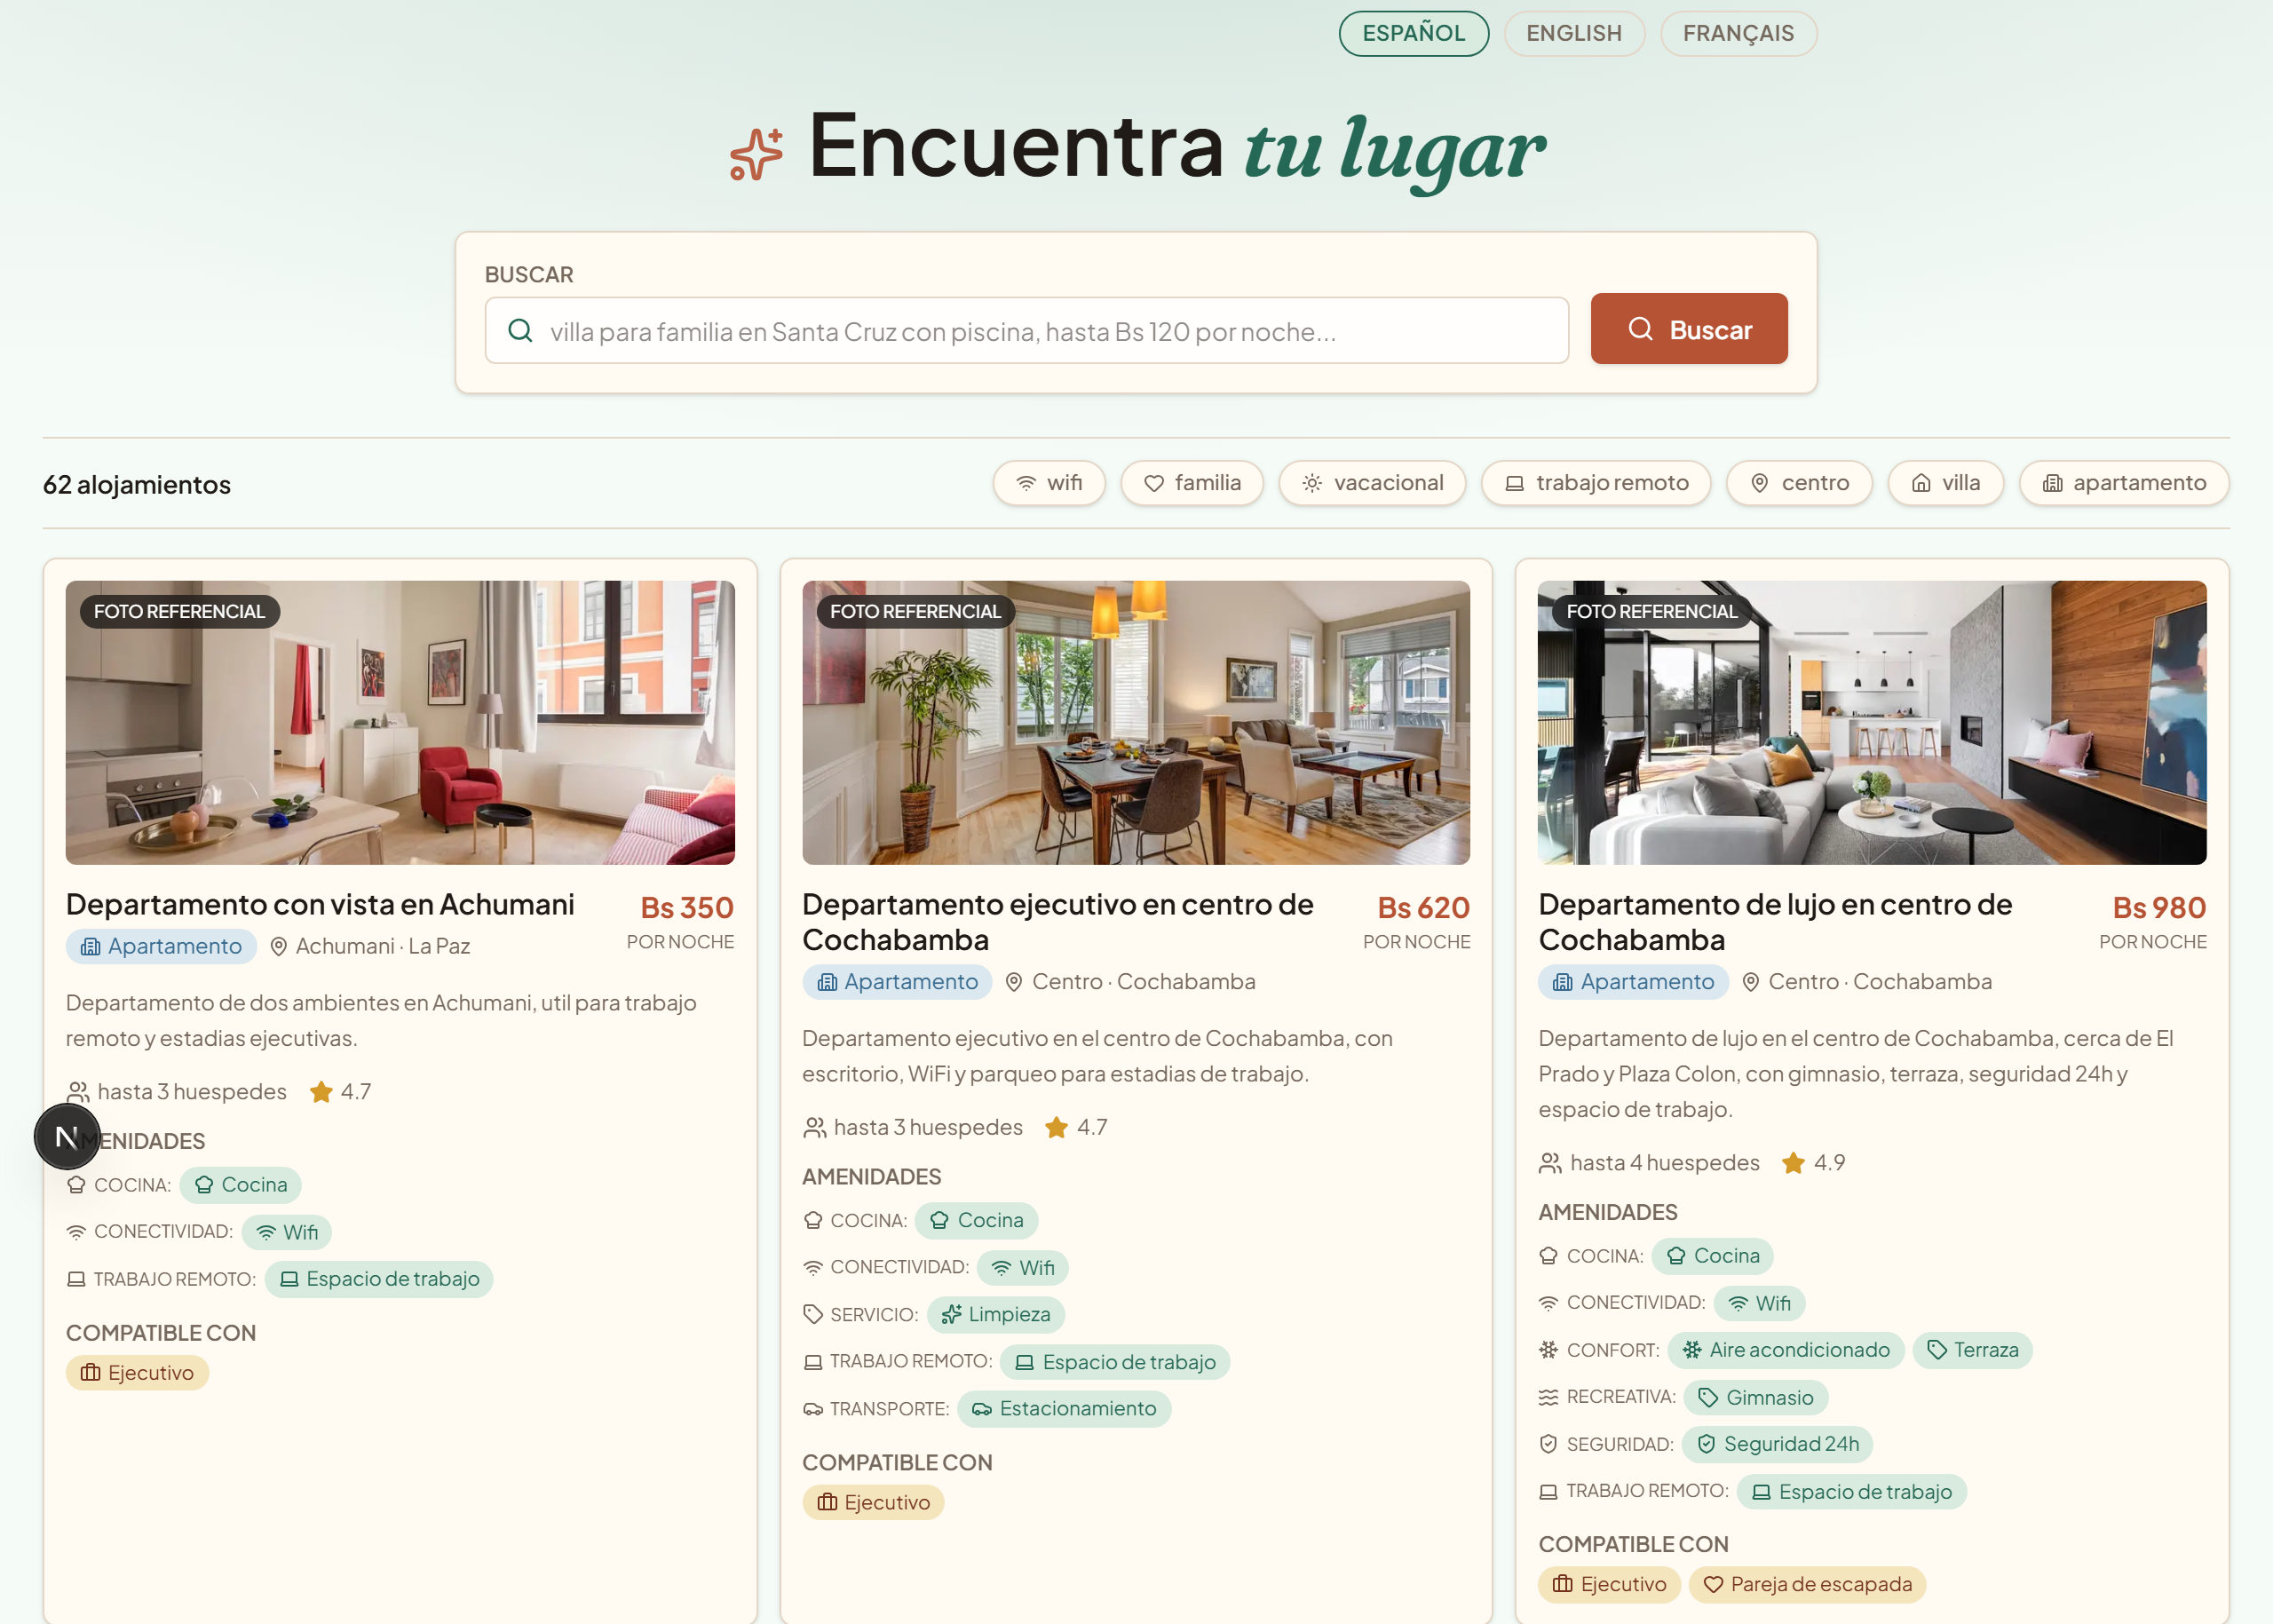
\includegraphics[width=0.9\textwidth]{images/ui_inicio_es.png}
\caption{Pantalla principal del buscador semántico en español.}
\label{fig:ui-es}
\end{figure}

\begin{figure}[H]
\centering

\includegraphics[width=0.9\textwidth]{images/ui_inicio_en.png}
\caption{Pantalla principal del buscador semántico en inglés sobre el mismo dataset OWL.}
\label{fig:ui-en}
\end{figure}

\begin{figure}[H]
\centering

\includegraphics[width=0.9\textwidth]{images/ui_inicio_fr.png}
\caption{Pantalla principal del buscador semántico en francés sobre el mismo dataset OWL.}
\label{fig:ui-fr}
\end{figure}

\begin{figure}[H]
\centering
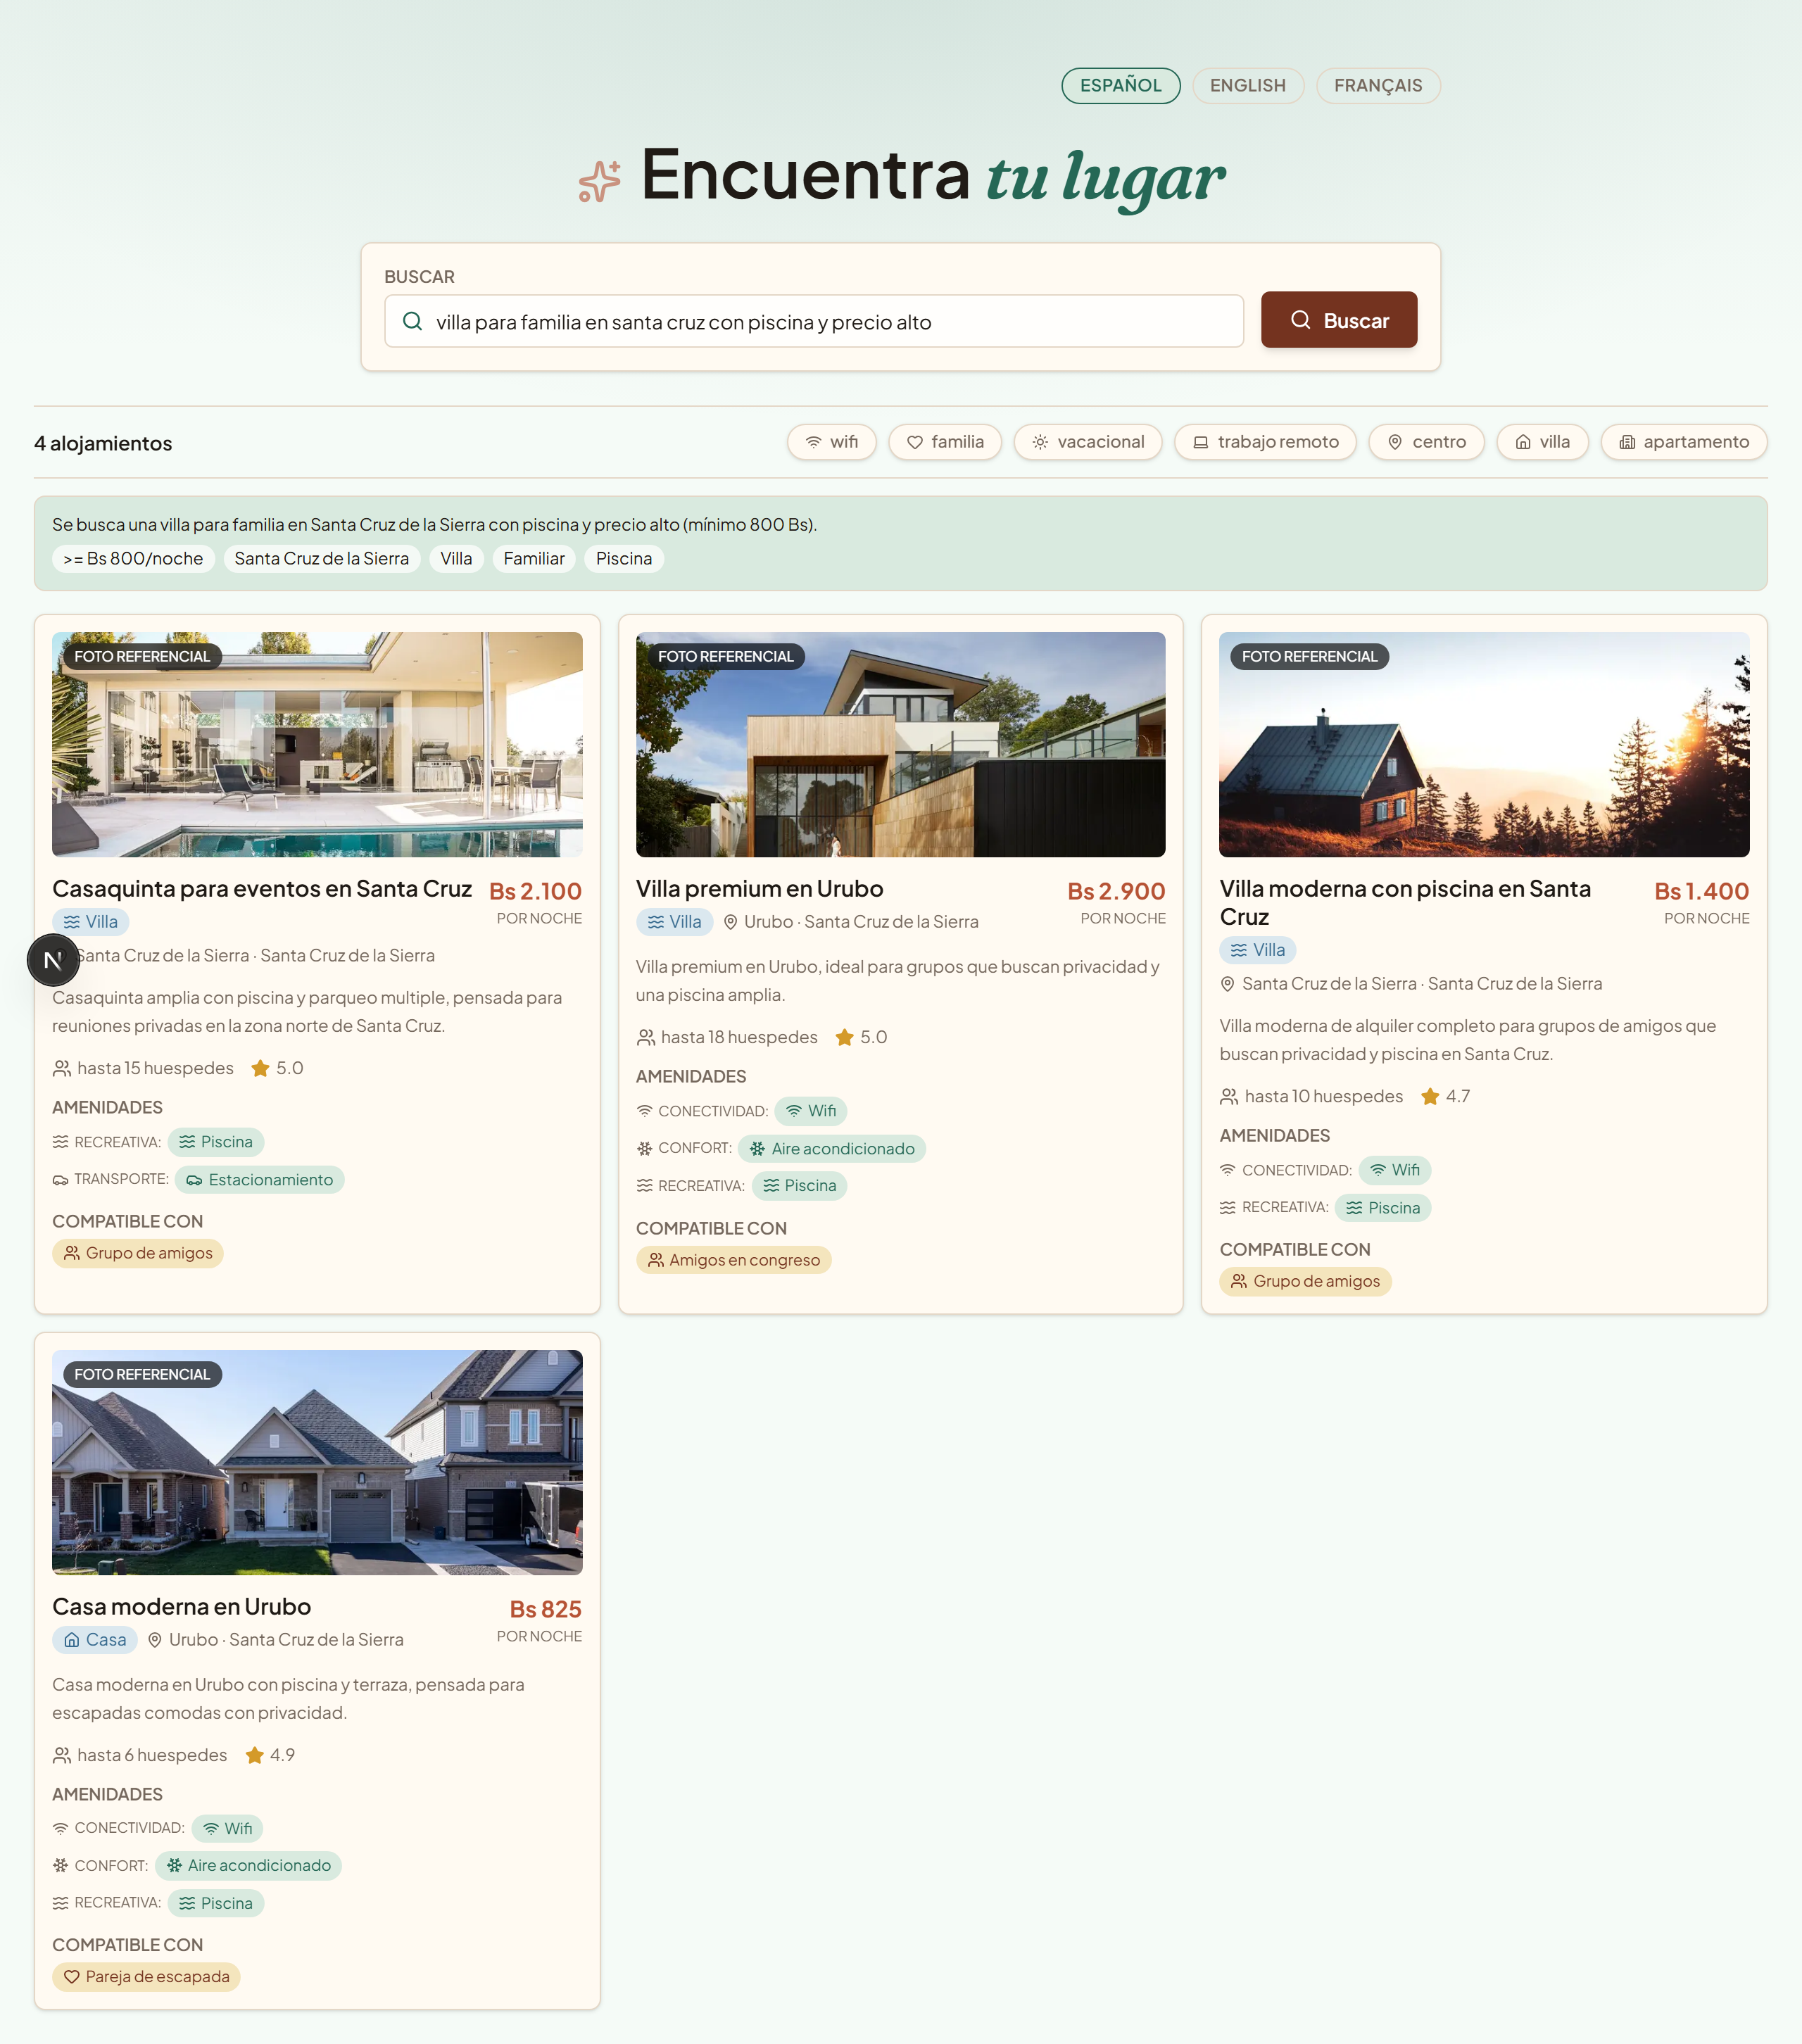
\includegraphics[width=0.9\textwidth]{images/ui_busqueda_compleja_es_1.png}
\caption{Resultado de una búsqueda compleja en español orientada a villas familiares en Santa Cruz con piscina y sesgo de precio alto.}
\label{fig:ui-es-compleja-1}
\end{figure}

\begin{figure}[H]
\centering
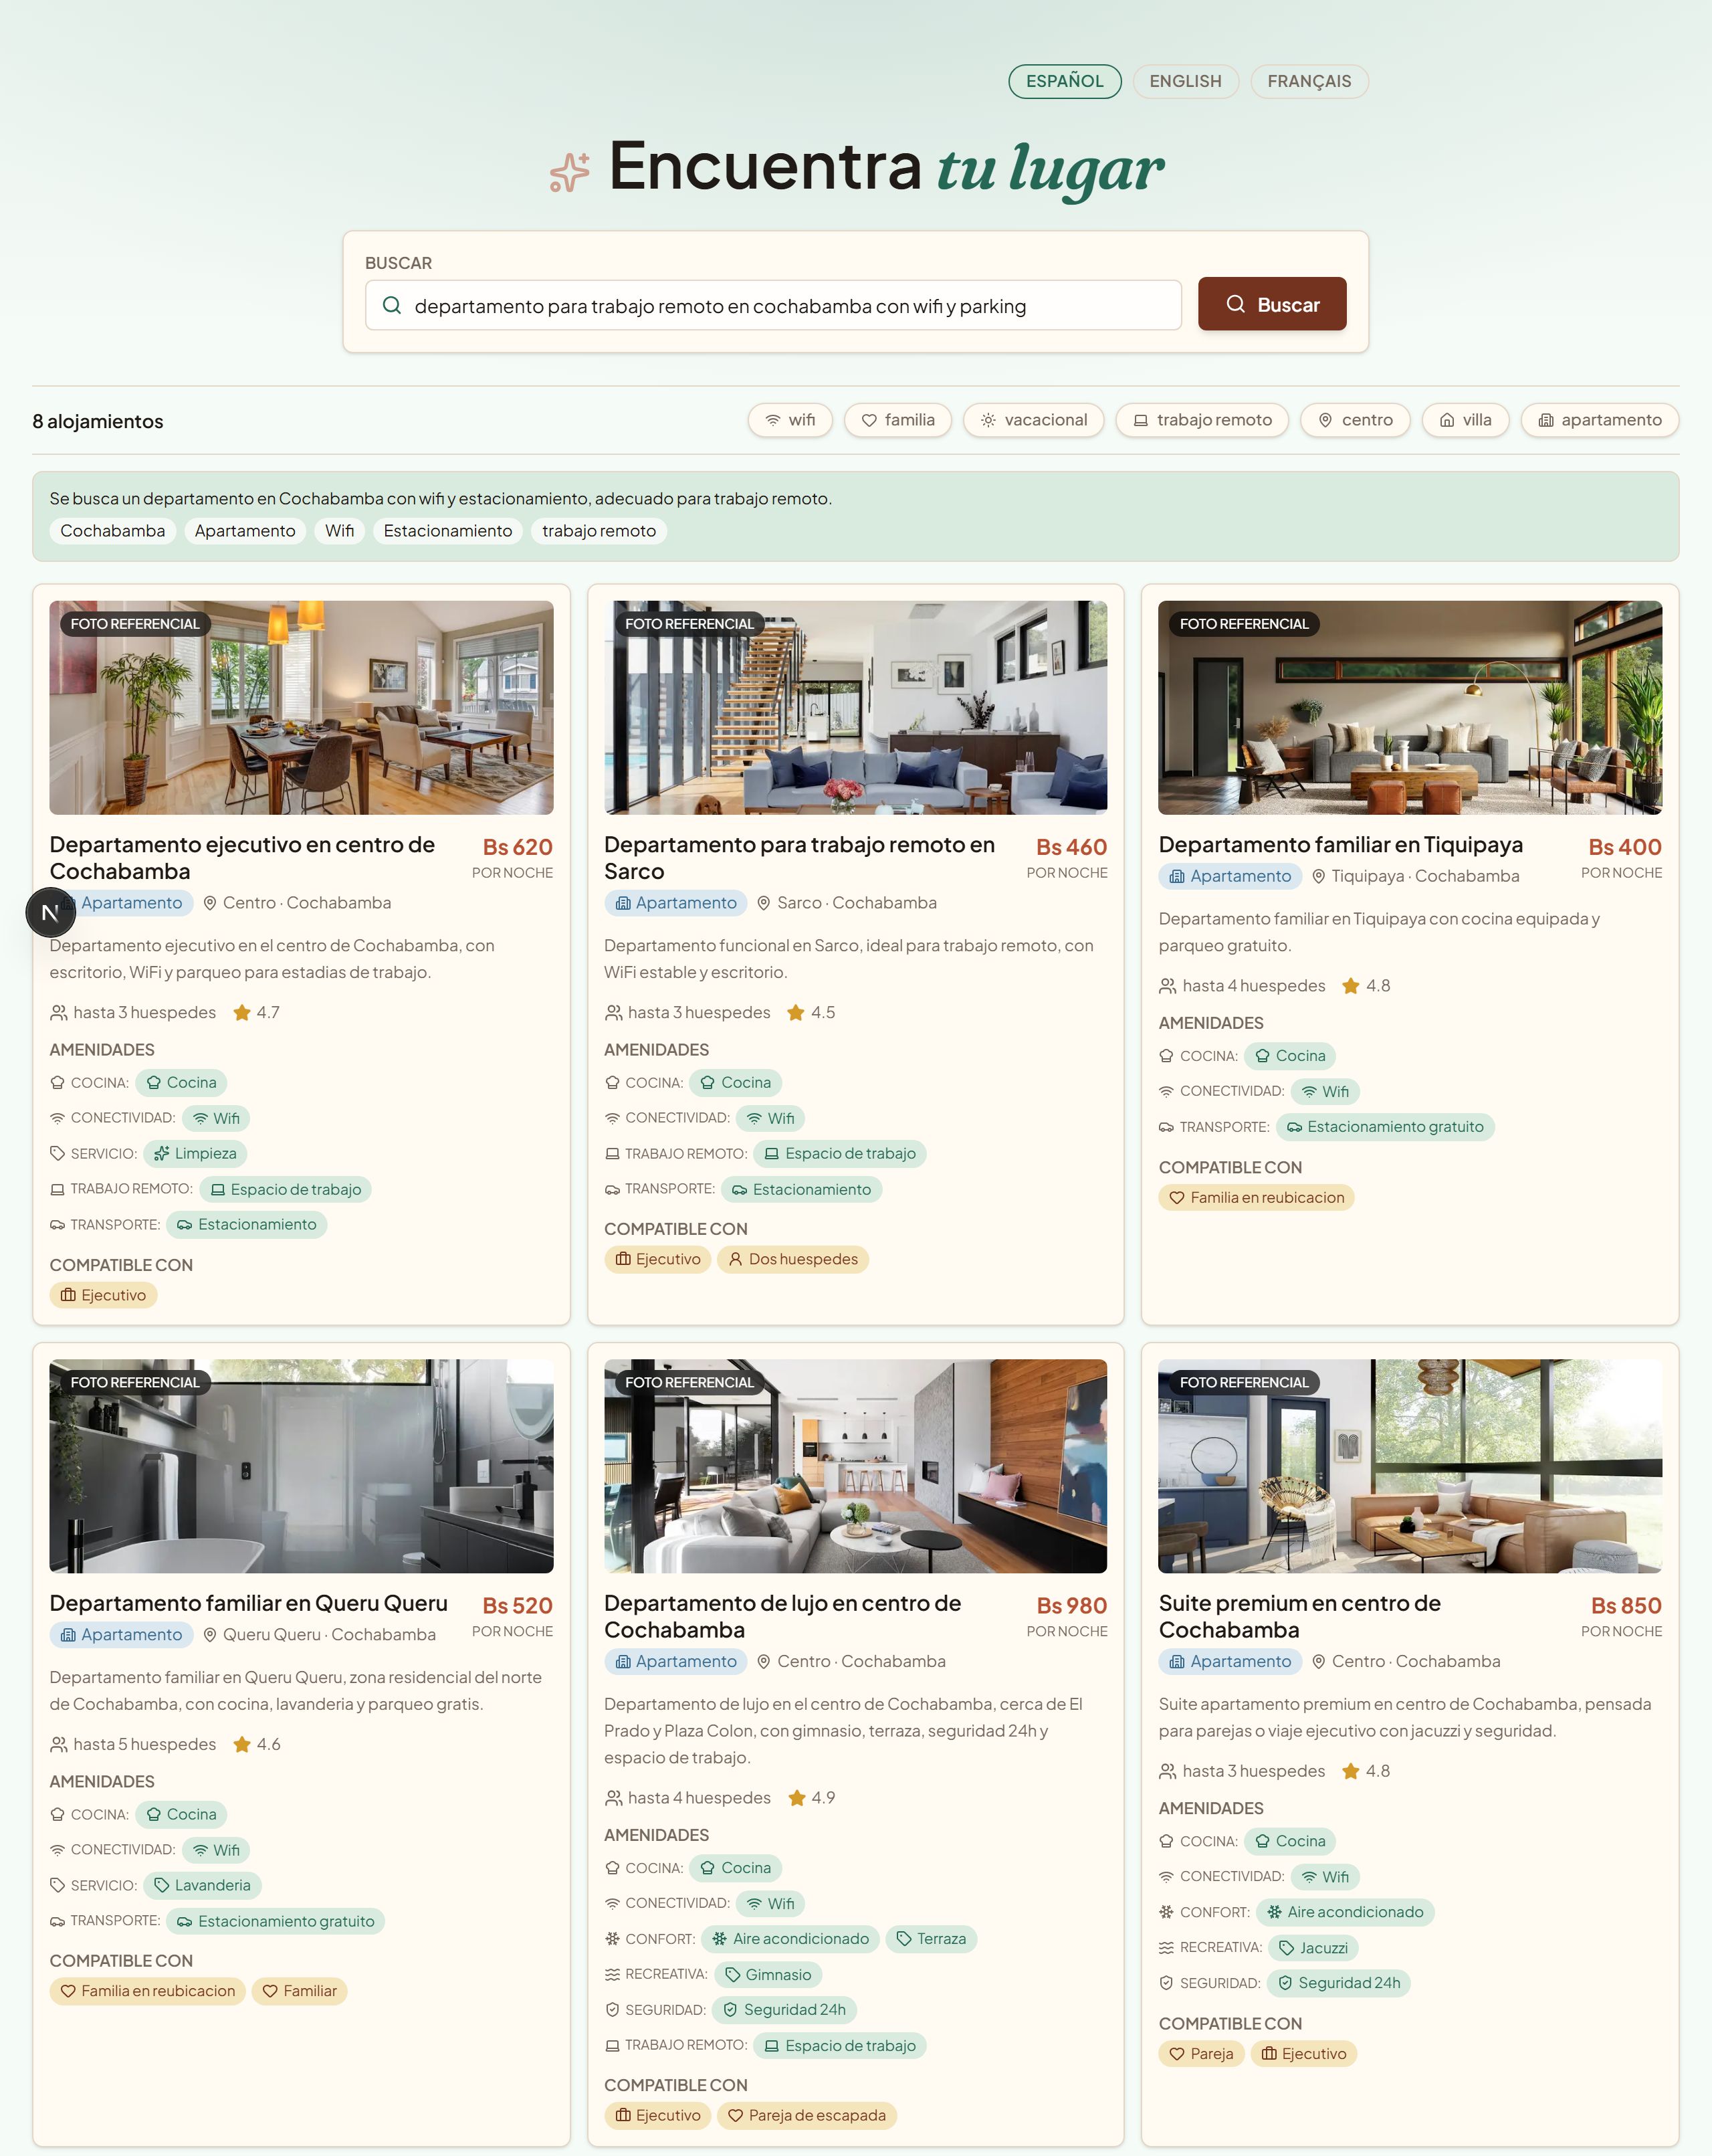
\includegraphics[width=0.9\textwidth]{images/ui_busqueda_compleja_es_2.png}
\caption{Resultado de una búsqueda compleja en español orientada a trabajo remoto en Cochabamba con Wi-Fi y estacionamiento.}
\label{fig:ui-es-compleja-2}
\end{figure}

\begin{figure}[H]
\centering
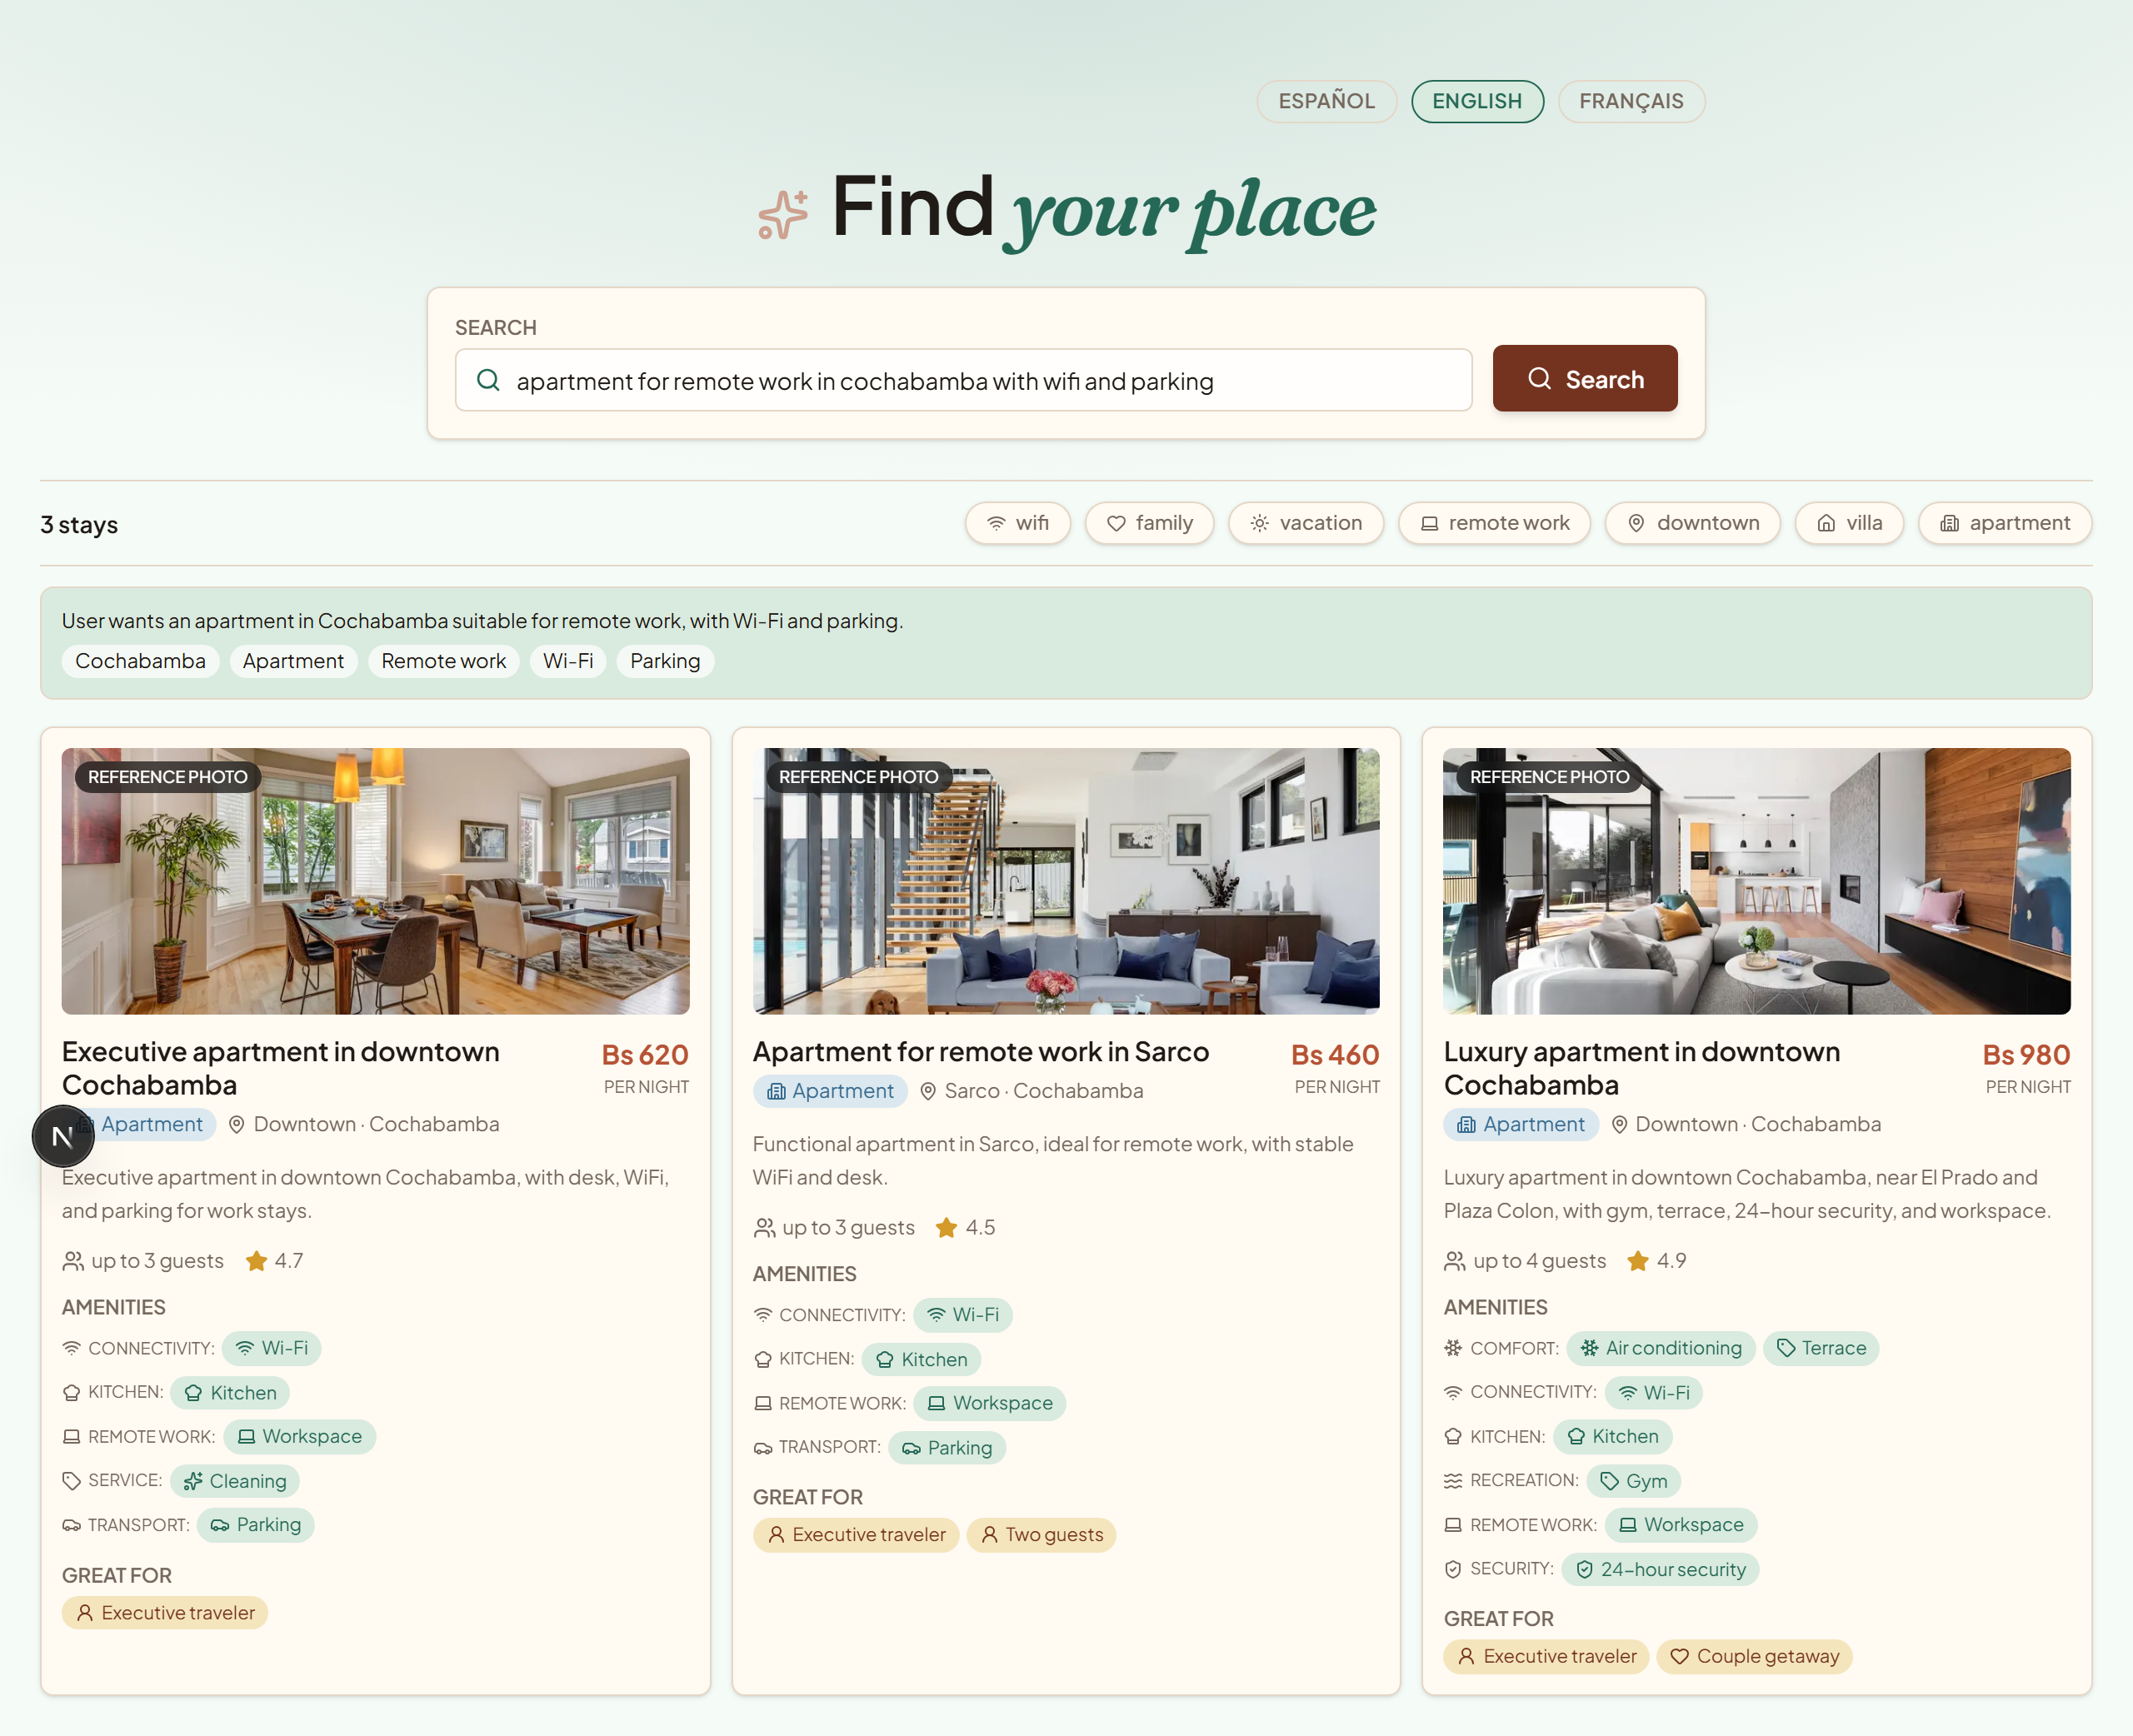
\includegraphics[width=0.9\textwidth]{images/ui_busqueda_compleja_en_1.png}
\caption{Resultado de la misma intención de búsqueda compleja en inglés, evidenciando recuperación semántica multilingüe.}
\label{fig:ui-en-compleja-1}
\end{figure}

\subsection{Valor técnico del prototipo}

La principal aportación técnica del sistema es demostrar que una ontología OWL puede ser
el centro operativo de un prototipo moderno de búsqueda, y no solo un modelo teórico.
La solución integra representación formal, consulta semántica, enriquecimiento con
Linked Data, multilingüidad real y una interfaz web usable. En consecuencia, el
proyecto cumple con el objetivo de aplicar investigación de Web Semántica en un
artefacto de software funcional, defendible y alineado con el enunciado de la práctica.


\clearpage
\section{CONCLUSIONES}

El desarrollo del buscador semántico permitió comprobar que las tecnologías de la Web
Semántica resultan adecuadas para modelar dominios de alojamiento temporal donde la
información relevante no puede reducirse a filtros aislados. La ontología construida en
OWL/RDF representó de forma coherente propiedades, amenidades, perfiles de huésped,
propósitos de viaje, políticas y contexto geográfico, habilitando consultas más
expresivas que las disponibles en un catálogo convencional.

La integración con DBpedia cumplió un doble propósito. Por un lado, aportó una base
externa confiable para enlazar tipos de alojamiento, amenidades y ciudades bolivianas
mediante \texttt{owl:sameAs} y \texttt{owl:equivalentClass}. Por otro lado, permitió
justificar la interoperabilidad del proyecto con el ecosistema de \textit{Linked Data}
sin comprometer la estabilidad del prototipo, dado que la operación principal se ejecuta
sobre un dataset local en Fuseki.

La implementación de multilingüidad mediante \texttt{rdfs:label} y
\texttt{rdfs:comment} demostró ser una decisión técnicamente sólida. A partir de un
único grafo RDF fue posible publicar y recuperar resultados en español, inglés y
francés, evitando duplicación de entidades y manteniendo una representación semántica
consistente entre idiomas. Esta estrategia confirma la ventaja de RDF/OWL para soportar
internacionalización de forma nativa.

Desde la perspectiva de ingeniería, el uso de Fuseki como \textit{triple store}, SPARQL
como lenguaje de consulta y Next.js como capa de presentación permitió construir un
prototipo funcional y cercano a un escenario real de uso. El sistema no quedó limitado
a la teoría ontológica: ofrece interfaz web, resultados visuales, navegación por idioma
y un flujo de búsqueda operable por el usuario final.

La validación con HermiT y las pruebas funcionales realizadas muestran que la solución es
coherente tanto en el plano lógico como en el operativo. En consecuencia, se concluye
que el objetivo de la práctica fue alcanzado: se desarrolló un buscador semántico basado
en OWL/RDF, enriquecido con DBpedia, con soporte multilingüe y materializado en una
aplicación de software defendible académicamente.

Como trabajo futuro, el proyecto puede ampliarse con nuevas ciudades, más puntos de
interés, consultas geográficas basadas en coordenadas, reglas de razonamiento más ricas
y un módulo de administración de datos que permita poblar la ontología de forma más
automatizada. Sin embargo, aun en su estado actual, el prototipo constituye una prueba
completa de aplicación de técnicas de Web Semántica en un problema concreto del dominio
de alojamiento temporal.


\clearpage
\printbibliography[title={BIBLIOGRAFÍA}]

\end{document}
